\documentclass [11pt, a4paper, oneside, article]{memoir}

%Inhaltsverzeichnis:
\usepackage{hyperref} %for hyperlinks
\maxtocdepth{section} %for depth in contents

%subsection numbering showed:
\setsecnumdepth{subsection}

%Including PDFs
\usepackage{pdfpages}

%Font: Arial
\usepackage{helvet}
\renewcommand{\familydefault}{\sfdefault}

% wenn unbekannte Silbentrennung dann in nächste zeile und große abstände
\sloppy

%Zeilenabstand:
\OnehalfSpacing

%Abstände zum Rand:
%TODO:
%\setlrmargins{1in}{*}{*}
%\setulmargins{0.6in}{0.6in}{*}

%Umlaute erlauben
%\usepackage[utf8]{inputenc

%Inserting Images:
\usepackage{graphicx}
\graphicspath{ {./images/} }

%For Highlighting Commands
\usepackage{listings}
\lstset{basicstyle=\tiny}

%Bibliography: APA
\usepackage{apacite}
\bibliographystyle{apacite}
% Change Caption language
\renewcommand{\figurename}{Abbildung}
\renewcommand{\figurerefname}{Abbildung}
\renewcommand{\contentsname}{Inhaltsverzeichnis}
%TODO: doesnt work:
\renewcommand{\bibname}{Literaturverzeichnis}


\begin{document}

%\frontmatter
\mainmatter

\includegraphics[scale=0.07]{Logo_Uni-Kassel.png}\vspace{50pt}
\begin{center}
\textbf{Universität Kassel}\\
Fachbereich Maschinenbau\\\vspace{50pt}
\textbf{Portfolio}\\
Studiengang: Mechatronik\\\vspace{20pt}
\textbf{Fach: Wissenschaftliches Schreiben und Präsentieren für MechatronikerInnen}\\\vspace{50pt}

\begin{tabular}{rl}
Verfasser: & Johannes Hölker\\
 & Matr.-Nr. 35192059\\
 & Kattenstraße 9\\
 & 34119 Kassel\\
 & johannes.hoelker@uni-kassel.de\\\vspace{40pt}
 & \\
 & \\
 & Kassel, den 20. März 2021\\
\end{tabular}
\end{center}

\tableofcontents*
\chapter{Einleitung}
Diese Sammlung an Texten dient dem Bestehen des Kurses "Wissenschaftliches Schreiben und Präsentieren für Mechatronik", welcher im Wintersemester 2021/2022 von dem Verfasser belegt wurde.\\
Bei wöchentlichen Abgaben wurden Kenntnisse und Fähigkeiten im Verfassen wissenschaftlicher Texte und Arbeiten geübt und vertieft. Die entstandenen Aufsätze sind in überarbeiteter Version in diesem Portfolio zusammengefasst. \\
Die jeweiligen Rohversionen sind im Anhang zu finden, teils mit markierten Verbesserungen, welche in Partnerarbeit entstanden sind.\\
Die Inhalte der Texte befassen sich vorwiegend mit dem Klimawandel und der Frage, wie dieser mithilfe von unterschiedlichen Technologien und Aktionen auf ein bestimmtes Maß begrenzt werden kann. Dabei wird zum Beispiel über Elektromobilität und erneuerbare Energien gesprochen.\\
Des weiteren gibt es Aufsätze zu dem Studiengang Mechatronik und zu im Körper eingepflanzten Chips, eine Artikelrezension mit dem Thema Bewegung eines Roboterarms, eine Prozessgrafik zu einem Kaufprozess und abschließend eine Projektskizze zu einer Bachelorarbeit.
%TODO: was für BA


\chapter{Hausaufgaben}
\section{HA 01: Warum sollte man Mechatronik studieren?}
  Computer, Auto, Smartphone, nahezu jedes Gerät aus deinem Alltag funktioniert so wie du es willst... Aber wie ist das möglich? Diese technischen Zusammenhänge zu erkennen und zu verstehen bringt der Studiengang Mechatronik mit sich.\\
  Im Grundstudium lernt man die Grundlagen aus den technischen Teilbereichen Maschinenbau, Elektrotechnik und Informatik kennen. Anschließend wird auf die Symbiose dieser Bereiche eingegangen und am Ende kann man sich nach den eigenen Interessen richten und sich spezialisieren. So werden dir im Laufe des Studiums die Abläufe vieler technischer Geräte und Prozesse klar.\\
  Dieses breit gefächerte Wissen ist nach abgeschlossenem Studium in deinem Repertoire und man hat anschließend die freie Wahl, auf welchen Fachbereich man sich nach dem Mechatronikstudium spezialisieren möchte oder ob man Schnittstellen der Fachbereiche koordiniert.\\
  Lass dir nach deinem Abitur nicht die Möglichkeiten nehmen und fokussiere   dich nicht zu früh auf einen Fachbereich, denn wer weiß welche Interessen du nach dem Studium haben wirst. Der Bachelor in Mechatronik qualifiziert dich für den Master in nahezu jedem technischen Zweig, sowie natürlich für einen Master in Mechatronik.\\
  Wenn deine Stärken in der Mathematik oder der Physik liegen bist du bei Mechatronik genau richtig. Aber auch wenn du nicht viel Vorerfahrung hast, kann der Studiengang Mechatronik was für dich sein. Du lernst die Grundlagen neu kennen und sie anschließend anwenden. Die Themen werden sehr grundsätzlich erklärt und mit dem nötigen Interesse kann man auch fachfremd in das Studium einsteigen.

\section{HA 02: Welche Technologie wird in den nächsten 5 Jahren von immenser Bedeutung sein?}
%„Überleitung von der Einleitung verbessern. Hier habe ich das gefühl das ich plötzlich reingeworfen werde “ zb Unsere welt wird häufiger von umweltkatasprophen heimgesucht , was auf die Erderwärmung zuruck zu führen ist....
  Um die Lebensgrundlagen der Menschheit und aller weiteren Tierarten nicht weiter zu gefährden und zu zerstören, darf die globale Erderwärmung keine 1,5° Celsius überschreiten \cite{masson-delmotte_ipcc_2019}.\\
  Um die schon jetzt auftretenden Folgen des anhaltenden Klimawandels noch stoppen zu können, kann an vielen unterschiedlichen Stellen etwas getan werden. Dazu gehört unter anderem der Verkehrssektor, der Ernährungssektor und vor allem der Energiesektor. Weltweit ist der Energiesektor der größte Emittent von Treibhausgasen, die Verbrennung fossiler Brennstoffe beträgt 88\% der CO2-Emmissionen, und das muss sich zwangsläufig und innerhalb kurzer Zeit ändern \cite{quaschning_regenerative_2019}.\\
  Die nötigen Mittel das zu erreichen haben die Menschen schon erfunden. Mit Solar- und Winkraftanlagen gibt es zwei ausgereifte Technologien, welche saubere Energie liefern. Diese Energieproduzenten können in Deutschland, sowie auf der ganzen Welt errichtet werden. \\
  Jedes Hausdach kann potenziell ein Solarkraftwerk werden. Deshalb sollte bei Neubauten auf eine Abdeckung mit Solarplatten geachtet werden. Die Technologie ist insofern ausgereift, dass die aktuell zum Verkauf stehenden Solarplatten technisch nicht mehr verbessert werden können. Lediglich eine thermische Nutzung mit Wasser kann den Wirkungsgrad noch erhöhen. Das erwärmte Wasser kann dann für die Heizung oder das Warmwasser genutzt werden.\\
  Noch nicht ausgereift ist die Energiespeicherung. Diese ist essentiell für eine erfolgreiche Energiewende. Das bedeutet, dass unsere Nutzung von Energie sich zwangsläufig an die Energiegenerierung anpassen muss. Nur wenn die Sonne scheint und der Wind weht, wird Energie generiert und bei einem Überschuss werden die Akkus geladen. Wenn diese irgendwann leer sein sollten, kann auch keine Energie mehr bezogen werden.\\
  Ein großer Vorteil der Technologie Solar ist die Möglichkeit der dezentralen Verteilung. Mit einem weit verbeiteten Netz aus vielen Akkus, welche sich dann gegenseitig unterstützen, kann trotzdem eine durchgehende Versorgung gewährleistet werden. Erst durch die polyzentral verteilte Generierung und Speicherung von Solarstrom, welche durch Batteriestationen in jedem Haus erreicht wird, können wir unabhängig von fossilen Energieträgern werden.\\
  %"Unabhängig werden" ist dabei ein zentraler Begriff. Ohne die Verlegung von langen Leitungen kann ein Haushalt in der Peripherie mit einer sogenannten Inselnetzanlage autark mit Strom versorgt werden.
  %An das Netz gekoppelte Systeme dagegen bekommen den überschüssigen Strom ausbezahlt, das macht einen Hausbesitzer/ eine Hausbesitzerin mit großer Dachfläche zu einem Energielieferanten und im besten Fall kann man davon sogar leben.

\include{Hausaufgaben/3_Elektromobilitaet/Elektromobilität_Johannes}
\section{HA 04: Erneuerbare Energien} \label{ha04}
% Drastische Einleitung
  Das 1,5-Grad Ziel ist aktuell nur noch schwer zu erreichen. "Eine globale Erwärmung von 1.5\textcelsius\ und 2\textcelsius\ wird im Laufe des 21. Jahrhunderts überschritten werden, es sei denn, es erfolgen in den kommenden Jahrzehnten drastische Reduktionen der CO2- und anderer Treibhausgasemissionen." \cite{ipcc_climate_2021}. Die entstehenden Extremwetterereignisse wirken sich auf die gesamte Erde aus. Um das zu verhindern ist es für jeden Menschen relevant, etwas dafür zu unternehmen die Erderwärmung zu begrenzen.\\
% Treibhausgasemittenten:
  Der größte Emittent von Treibhausgasen ist der Energiesektor mit einem Anteil von 73,2\%, gefolgt von der Nahrunsgmittelproduktion mit 18,4\% \cite{ritchie_co_2020}. Deshalb ist es immens wichtig im grösten Sektor der Treibhausgasemmissionen nach klimafreundlicheren Lösungen zu suchen, was bedeutet erneuerbare Energien zu fördern.\\
% Energiesektor:
  Dass der Energiesektor einen so hohen Anteil an den Treibhausgasemmissionen hat liegt neben dem enorm hohen Konsum von Energie in der heutigen Zeit daran, dass 2020 85\% des weltweiten Primärenergiebedarfs klimaschädliche Energieträger lieferten \cite{quaschning_regenerative_2019}. Die Verbrennung von Kohle, Erdöl und Erdgas trägt demnach maßgeblich zur globalen Klimakatastrophe bei und das muss geändert werden.\\
% Lösungsansatz erneuerbare
  Ändern kann man dies urch den Einsatz von erneuerbaren Energien. Die Sonne liefert jeden Tag soviel Energie, dass allein die Fläche der Sahara ausreichen würde die 200-fache weltweit benötigte Energie zu liefern. Die Nutzung der Energie, welche auf die Fläche Niedersachsens trifft, würde demnach den weltweiten Energiebedarf decken \cite{quaschning_regenerative_2019}.\\
% wie nutzt man sonnenenergie?
  Die direkte Nutzung von Sonnenstrahung ist mithilfe von Photovoltaik möglich. Solarzellen, welche mithilfe des Photoeffekts sehr hohe Wirkungsgrade erzielen, können immer dann Strom erzeugen, wenn es hell ist. Indirekt wird die Sonnenenergie über Wind oder Wasserkraft genutzt. Wie bei Photovoltaik kann auch hier nur dann Strom erzeugt werden, wenn der Wind weht oder genug Wasser zum Antribe von Turbinen vorhanden ist. Die Entwicklung dieser Technologien ist weit fortgeschritten, sodass sie im großen Stil eingesetzt und lange betrieben werden können \cite{quaschning_regenerative_2019}.\\
% Energiespeicher:
  Scheint keine Sonne oder weht kein Wind, stoßen  erneuerbare Energien jedoch auf ein zentrales Problem, denn dann liefern sie keinen Strom mehr. Um die Versorgungslücke zu schließen, muss demnach Energie als Puffer zwischengespeichert werden. Die Entwicklung von Energiespeicherlösungen ist dabei noch nicht ausgereift und die Herstellung handelsüblicher Batterien erfordert den Einsatz von Ressourcen, die nur schwer zu erreichen sind.\\
% Fokus der Forschung:
  Demnach sollte im Fokus der Forschung die Entwicklung neuer nachhaltiger Energiespeicher stehen. Des Weiteren ist der schnelle Aufbau von erneuerbaren Energiegeneratoren wichtig. Die Frage ist nicht, wie können wir die Technologien verbessern, sondern wie können wir so viele von den bestehenden Technolgien so schnell wie möglich in der Praxis einsetzen und aufbauen.\\
% Lösungsansätze:
  Um den Einsatz von Menschen zu verringern und die Effizienz von arbeitenden Elektroinstallateuren und Ingenieuren zu erhöhen, kommen Entwicklungen in der Automatisierung und Planung durch KI-Systeme in Frage. Aber auch politische Entscheidungen und der Wille in der Bevölkerung tragen zur Energiewende bei. Erst wenn alle Akteure an einem Strang ziehen, kann die Klimakatastrophe vermieden werden.

\section{HA 05: Artikelrezension}
% Das wird behandelt:
  In dem Artikel von \cite{jiang_development_2017} "Development of a Motion Controlled Robotic Arm" wird ein technisches System vorgestellt, in welchem ein Roboterarm mit der menschlichen Armbewegung gesteuert wird. Dabei steht die technische Umsetzung im Vordergrund.\\
% Verortung im Forschungsdiskurs:
  Eine klare Begründung für den Bau und den Einsatz eines solchen Systems wird in der Einleitung mit der Aussage des Einsatzes in gefährlichen Bereichen geliefert. Eine wissenschaftliche Recherche, inwieweit das entwickelte System schon von anderen gebaut wurde oder diverse Vorgänger besitzt, wurde dabei nicht durchgeführt.\\
% Gelungen:
  Die Hardware, bestehend aus dem Arduino Uno, 4 Servomotoren und diversen Sensoren wird eingehend erklärt und die Funktionsweise ist klar verständlich. Auch die Zusammensetzung der Komponenten ist ersichtlich. Zum Beispiel kann man gut nachvollziehen, wie die Stromversorgung ausgelegt wurde.\\
% Unverständlich/ Fehlerhaft/ Unverständlich und offene Fragen:
  Die Beschreibung der Software ist dagegen wenig ausführlich. Es wird erwähnt welche Ein- und Ausgaben der Mikrocontroller hat und wie die Positionierung des Roboters mithilfe des Kompasses abläuft. Dabei bleibt aber unklar, wie die Berechnung der einzelnen Winkel für die Servomotoren aussieht und wie sie programmatisch umgesetzt wurde. Dies wird nur mit einem Satz erwähnt: "Additionally, two of the accelerometer outputs are used to determine the vertical angles that the bicep and the forearm of the robot should be at." Diese fehlende Information ist wichtig, da sie den Kern der Arbeit ausmacht und das größte zu lösende Problem darstellt.\\
  Des Weiteren wird nicht auf die Theorie eingegangen, welche hinter der Kinematik eines menschlichen Arms steht. Das wäre bezüglich der Auswahl der Servomotoren relevant gewesen und bleibt ungeklärt.
%TODO:

\section{HA 06: Welche Forschungsprojekte sollten an Universitäten in Zukunft stärker gefördert werden?}
% Einleitung:
  Naturbasierte Lösungen (NBL): So lautet einer der bei der COP in Glasgow genannten Ansatzpunkte, um den anhaltenden Klimawandel noch aufzuhalten. Die zentrale Forderung lautet dabei, die Natur in ihrer ursprünglichen Form zu schützen und schon vom Menschen beeinflusste Gebiete zu renaturieren \cite{wahnbaeck_nature-based_2021}. Es gibt verschiedene Wege NBL umzusetzen.\\
% Ansatzpunkt Uni:
  Universitäten bieten den Ansatz, Lösungen zu finden, sie weiterzuentwickeln und für die breite Masse anwendbar zu machen. Anschließend können Empfehlungen formuliert werden, welche von Politik und Unternehmen übernommen werden sollten. Die von der Wissenschaft erarbeiteten Lösungen sind dabei frei von subjektiven Meinungen und bieten eine Grundlage, auf derer die Politik Entscheidungen treffen kann.\\
% Forschung
  Um die passenden Empfehlungen für einen funktionierenden Klimaschutz zu bekommen, sollte dabei im Vorfeld in die richtige Richtung geforscht werden.\\
% Zitation Bund:
  Das Bundesministerium für wirtschaftliche Zusammenarbeit und Entwicklung (BMZ) hat bereits eine klare Haltung zu NBL und fördert proaktiv deren Einsatz. "Das in Wert setzen der Natur kann eine Schlüsselrolle spielen, um Klimaanpassung zu fördern und Katastrophenrisiken zu verringern." \cite{bundesministerium_fur_wirtschaftliche_zusammenarbeit_und_entwicklung_naturbasierte_2021} Aus diesem Grund ist nun die Wissenschaft gefragt.\\
% urbaner Wald
  Eine dieser NBL ist der urbane Wald, bzw. die allgemeine Begrünung von Städten. Diverse Vorteile ergeben sich dadurch: "Der Wald filtert die Luft, nimmt Regenwasser auf und kühlt die sich aufheizende Stadt in Zeiten der Klimakrise. Die Anwohner können Natur vor ihrer Haustür erleben. Und die Stadt spart Geld, das sie sonst in pflegeintensive Parks stecken müsste." \cite{wahnbaeck_nature-based_2021}.\\
  Ein aktueller Leitfaden der Universität Osnabrück liefert ein gutes Beispiel für die Formulierung von Empfehlungen. Dieser gibt Handlungsempfehlungen für Dachbegrünung in Innenstädten, welche direkt umsetzbar sind und der Stadtverwaltung, sowie Privatleuten helfen, ihre Dächer zu bepflanzen \cite{schroder_extensive_2020}.\\
% Stadtbegrünung
  Diesem Vorbild folgend, können tiefergehende Entwicklungen für die Begrünung von Städten entstehen, zum Beispiel technische Lösungen für die Bepflanzung von Schrägdächern, welche bei der Sanierung von Dachziegeln angewandt werden können. Da viele Dinge, wie Bewässerung und Pflege, sowie der Schutz der Bausubstanz beachtet werden müssen, ist hier Forschungspotential gegeben.\\
% Renaturierung:
  Nicht nur der urbane Raum bietet Möglichkeiten zur nachhaltiges Umgestaltung. Auch auf dem Land gibt es Potenzial für NBL. Die Renaturierung von Flussauen oder die Nutzungsänderung von landwirtschaftlich genutzten Flächen zu Forstflächen bieten ein großes Forschungsfeld. Die Erfassung von Tierarten und der Einfluss auf die Erholung der Bestände kann in langfristigen Studien erfasst werden.\\
% weitere Forschungspotentiale
  Gleichzeitig haben Universitäten die Möglichkeit, die Bevölkerung aufzuklären und Fakten zu schaffen. Aus einer Studie der Hochschule Bingen geht zum Beispiel hervor, dass Gründächer gegenüber Kiesdächern bezüglich Biodiversität, Mikroklima und Wasserhaushalt bedeutend wertvoller sind \cite{hietel_extensive_2016}.

\section{HA 07: fiktives Forschungsthema - implantierte Mensch-Maschine Schnittstelle}
\subsection{Einleitung:}
  Während sich viele Menschen nicht vorstellen können, elektrische Geräte in ihren Körper einzupflanzen, können andere nicht mehr ohne. Um die Gehirnaktivität zu messen und so fehlende Funktionen wie die Steuerung von Prothesen zu ermöglichen, werden im Gehirn eingepflanzte Chips schon verlässlich in der Praxis eingesetzt. Diese können mit der Peripherie kommunizieren und einfache Gedankengänge aufzeichnen.\\
  Das wirft die Frage auf, inwieweit die Technologie für die Bedienung eines Endgerätes verwendet werden kann. Dies würde die Notwendigkeit eines Touchscreens bei Smartphones beenden, womit das klobige Gerät langfristig wegfallen würde. Auch die Übertragungsgeschwindigkeit zwischen Mensch und Maschine würde drastisch erhöht werden (Musk, 2017). \\
  Ob diese Möglichkeit mit dem heutigen Stand der Technik erreicht werden kann, wird in dieser Arbeit untersucht. Dabei wird auf die Hilfsmittel eingegangen, welche aktuell schon genutzt werden und mit den verfügbaren Chips und den Studien zu diesen verglichen. Diverse Studien bestehen bisher zu einer Anwendung im Labor. Diese werden eingehend in Bezug auf gesundheitliche Sicherheit, Anwenderfreundlichkeit und Verlässlichkeit untersucht.\\
  Die konkrete Forschungsfrage lautet demnach:
  %Forschungsfrage:
  Sind eingepflanzte Chips alltagstauglich und können sie die Bedienung von Smartphones ersetzen?\\
  Die interdisziplinär auftretenden Probleme sind gleichzeitig in der Medizin, als auch der Informatik und Elektrotechnik verankert, was den umfangreichen Theorieteil nötig macht. Danach werden die analysierten Studien vorgestellt und im Anschluss auf die zu untersuchenden Punkte geprüft.
% Wird die Forschungsfrage aufgegriffen?
% Passen Einleitung und Fazit zusammen?
% Zusammenfassung der wesentlichen Erkenntnisse?
% Trichterprinzip?
\subsection{Fazit:}
  In der vorliegenden Arbeit konnte anhand der aktuellen Studienlage gezeigt werden, dass die Bedienung eines Smartphones mit Hilfe von im Körper eingepflanzten Chips prinzipiell möglich ist. Dies wurde in Pilotprojekten gezeigt. Eine Bedienung der gewohnten Funktionen wie wir sie kennen und ohne Probleme die im Alltag benötigten Anwendungen zu nutzen ist jedoch bisher nicht erreicht worden.\\
  Die Bedienung über kontrollierte Gedankenmuster konnte die Gesten auf einem Smartphone steuern. Diese Gesten haben ausgereicht, um Apps zu öffnen und voreingestellte Funktionen auszuführen (z.B. einen Anruf zu tätigen). Dies hat für bestimmte Fälle Vorteile gebracht, für eine alltägliche Nutzung waren diese Funktionen aber nicht weitreichend und detailliert genug.\\
  Die drei Forschungsgegenstände gesundheitliche Sicherheit, Anwenderfreundlichkeit und Verlässlichkeit wurden bei  durchgeführten Studien bewertet und fallen unterschiedlich stark aus. Es lässt sich keine allgemeingültige Bewertung ableiten, da größtenteils unterschiedliche technische Ansätze verfolgt wurden. Um die Forschungsfrage genauer zu beleuchten wären demnach die Betrachtung von einzelnen viel versprechenden technischen Ansätzen nötig, was in dieser Arbeit nicht gemacht wurde.\\
  Es lassen sich jedoch technische Teilbereiche ableiten, welche für die Umsetzung des Ziels nötig sind. Die Erkennung von Text und das "Diktieren" im Kopf muss sicherer und verlässlicher werden. Die Oberfläche für Smartphones, bzw das Bedienumfeld eines Chips im Kopf muss neu gedacht und pragmatisch neu festgelegt werden. Erst wenn feststeht, wozu Chips im Kopf genutzt werden sollen und die Chancen erkannt wurden, kann an der Entwicklung einer passenden Schnittstelle gearbeitet werden.
%(Zusammenfassung etwas kurz geraten, evtl noch mehr auf die Studienergebnisse eingehen. Außerdem fehlt die Bewertung der eigenen Arbeit. Ausblick und abschließender Satz gut)

%TODO: Grafik drehen und an Text anpassen

\section{HA 08: Beschreibung Kaufprozess Elektronikkauf}
  Bevor neue Elektronikgeräte gekauft werden, sollte man sich besonders lange mit der Frage beschäftigen: "Brauche ich das wirklich?" Der Aufwand an Ressourcen und Energie zur Herstellung des Produktes steht oft in keinem Verhältnis zu der sinnvollen Anwendung. Oft stehen die Geräte nach zweimaliger Benutzung im Schrank und dienen nur als Deko. Erst wenn das Gerät wirklich akut benötigt wird, sollte man meiner Meinung nach über einen Kauf nachdenken. In der schematischen Darstellung beginnt der Kaufprozess daher mit der Situation, in der ein bestimmtes Gerät benötigt wird.\\\\
  Ist die Situation eingetreten, bei der die gewünschte Elektronik wirklich benötigt wird, lässt sie sich in vielen Fällen leihen oder mieten. Eine weitere Alternative ist der Gebrauchtkauf, bei der weniger Geld ausgegeben und nachhaltiger gehandelt wird.\\\\
  Tritt wiederholt der Fall ein, dass das Gerät gebraucht wird und Mieten und Gebrauchtkauf nicht in Frage kommen, sollte man sich über das Angebot der unterschiedlichen Anbieter eingehend informieren um einen Fehlkauf zu vermeiden. Ist dann teils aus dem Bauchgefühl und teils auf einer subjektiven Entscheidung heraus das passende Gerät gefunden, kann noch nach Vergünstigungen und in unterschiedlichen Läden, online wie offline, gesucht werden um das perfekte Angebot zu finden.\\
  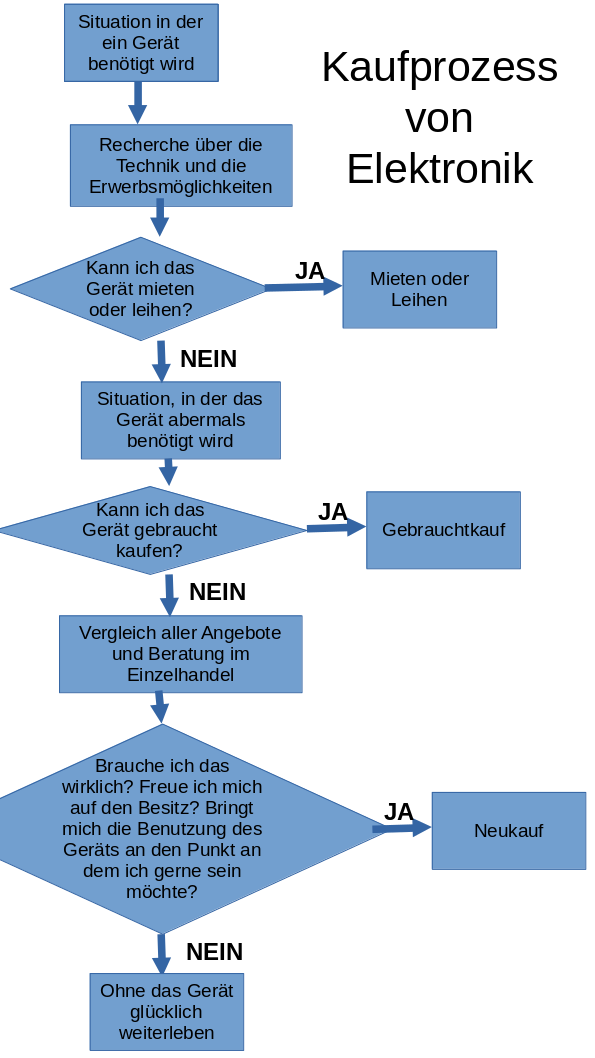
\includegraphics[scale=0.6]{Hausaufgaben/8_Kaufprozess/Kaufprozess_Grafik.png}


\section{HA 09: Projektskizze einer Abschlussarbeit}
\subsection{Deckblatt}

\includegraphics[scale=0.07]{Logo_Uni-Kassel.png}\vspace{50pt}
\begin{center}
\textbf{Universität Kassel}\\
Fachbereich Maschinenbau\\
Arbeits- und Organisationspsychologie\\\vspace{50pt}
\textbf{Bachelorarbeit}\\
Mechatronik\\\vspace{20pt}
\textbf{Intuitive Telepräsenzsteuerung eines anthropomorphen Manipulators unter Verwendung von Head-Mounted Displays und Motion-Capturing}\\\vspace{30pt}
\begin{tabular}{rl}
Betreuer: & Prof. Dr. phil. habil. Oliver Sträter\\
 & Dipl. Ing. M.Sc. Mehrach Saki \\
  & \\
Verfasser: & Johannes Hölker\\
 & Matr.-Nr. 35192059\\
 & Kattenstraße 9\\
 & 34119 Kassel\\
 & johannes.hoelker@uni-kassel.de\\\vspace{40pt}
 & \\
 & \\
 & Kassel, den 20. März 2021\\
\end{tabular}
\end{center}

\includepdf[pages=2-3]{./Hausaufgaben/9_Projektskizze_BA/main.pdf}
\section{Fragestellung}
%Wird einem potenziellen Betreuer ersichtlich, woran ich forschen möchte?
%Sind meine Ausführungen überzeugend und helfen sie, mein Thema zu "verkaufen"?
%Problemstellung:
  Die Programmierung und Steuerung von Manipulatoren geschieht aktuell noch über ein Umdenken des Anwenders indem er von einer anderen Perspektive auf das System schaut und es so steuert. Das kann Komplikationen erzeugen, erfordert Einarbeitung und Erfahrung und macht die Werkzeugtransformation schwierig. Um die fortschreitende Automatisierung für eine breite Masse verfügbar zu machen, müssen Manipulatoren intuitiv bedienbar sein. \\
%Zielsetzung:
  Ein System, was die Technologien der Robotik und der Datenbrillen kombiniert, kann helfen diese Problematik zu lösen. Durch Einsatz von Telepräsenz soll die anwendende Person die Perspektive des Roboters einnehmen und den Roboterarm intuitiv steuern können. \\
%Forschungsfrage:
  Die in dieser Arbeit behandelte Forschungsfrage lautet demnach:
  Wie lässt sich ein System mit den beiden Technologien Robotik und Datenbrillen bauen, um funktionierende Telepräsenz zu erreichen und so eine intuitive Steuerung eines Manipulators zu ermöglichen?

\subsection{Textprobe: vorläufige Einleitung}
%Ist der Text verständlich?
%Einhaltung sprachlicher und formaler Standards
  Zu Beginn dieser Arbeit wird die Motivation erläutert, aus welcher diese heraus geschrieben wird. Anschließend leitet sich daraus die Zielstellung ab und ein Überblick über die folgenden Kapitel wird präsentiert.
\subsubsection{Motivation}%Warum möchte ich das erforschen?
  Der erste ferngesteuerte Roboter, 1949 erfunden von Raymond Goertz, wurde dazu eingesetzt radioaktives Material gefahrenfrei zu bewegen. Die eingesetzte Methode des Master-Slave Manipulators übersetzte mechanisch die Bewegung des menschlichen Arms auf einen Manipulator. So konnten Gefahrengüter hinter einer durchsichtigen Trennwand bewegt werden. Dabei merkte Goertz an, dass die anwendende Person aus einem anderen Blickwinkel auf die auszuführende Aufgabe schauen muss und die Aufgabe so erschwert wird \cite{goertz_master-slave_1949}. \\\\
  Diese Problematik ist in der Robotik größtenteils durch eine Automatisierung der Manipulatoren gelöst worden. Durch ein hohes Maß an Sensorik und in kürzester Vergangenheit auch durch den Einsatz neuronaler Netze können sich Roboter weitgehend selbstständig bewegen \cite{siciliano_springer_2008}.\\\\
  % Ausführung von für den Menschen gemachten Arbeitsaufgaben
  Es gibt jedoch weiterhin viele Aufgaben, bei denen ein Mensch anwesend sein muss. Die Wartung von industriellen Maschinen, Pflegetätigkeiten und kooperatives Arbeiten sind nur ein paar Beispiele. Viele Arbeitsumgebungen sind des Weiteren für den Menschen konzipiert und die Aufgaben sind komplex und damit nicht direkt automatisierbar \cite{fritsche_first-person_2015}. Um dennoch die Aufgaben lösen zu können, ohne dass ein Mensch anwesend ist, kann ein anthropomorpher ferngesteuerter Manipulator eingesetzt werden \cite{tanie_mfi_2003}\cite{stanczyk_development_2006}.\\\\
  Herkömmliche Programmierverfahren erfordern des Weiteren viel Übung und Zeitaufwand. Die programmierende Person muss eine spezielle Ausbildung haben und braucht dennoch gewisse Zeit für die Umsetzung. Besonders in kleinen und mittelständischen Unternehmen bringen günstige Robotersysteme, welche einfach zu installieren, einzustellen, zu programmieren und zu warten sind, einen Vorteil. Um die genannten Arbeitsschritte zu vereinfachen erfordert es eine intuitive Steuerung des Roboters \cite[S.76]{brogardh_present_2007} \cite[S.190]{ehlers_echtzeitfahige_2019}. \\\\
  Räumlich in die Rolle des Roboters zu schlüpfen und aus der veränderten Perspektive heraus zu handeln eignet sich für eine Manipulatorsteuerung in für Menschen gefährlichen Umgebungen \cite[S.9]{mareczek_grundlagen_2020}. Diverse Konzepte und Systeme um diese Problematik zu lösen wurden entwickelt und werden in Kapitel 2 vorgestellt.\\\\
  % Mensch vor Technik:
  In der vorliegenden Arbeit wird demnach ein Arbeitsplatz gestaltet, welcher den Menschen mit Technik verbindet. Es werden Geräte eingesetzt, welche der Mensch tragen soll und so sein Umfeld beeinflussen. Für die gesamte Arbeitsgestaltung ist dabei wesentlich, dass nicht die technische Machbarkeit, sondern die "menschlichen Bedarfe und Möglichkeiten" im Vordergrund stehen \cite{strater_positionspapier_2019}. Für alle Entwicklungsschritte wird diese Richtlinie bedacht und evaluiert.\\\\
  % OpenSource für Nachhaltigkeit
  Aufgrund der aktuellen Situation des globalen Klimas \cite{ipcc_climate_2021}, soll die technische Entwicklung auch in Hinblick auf Nachhaltigkeit geschehen. Der Einsatz von Open Source Design (OSD) kann nach \cite{setchi_implications_2016} während und zum Ende des Lebenszyklus eines technischen Produkts einen positiven Einfluss auf Nachhaltigkeit haben. Die Reparierbarkeit, Wiederverwendbarkeit und die lokal-gebundene Wertschöpfung werden durch Ntzung von OSD ermöglicht und haben damit eine erhöhte Effizienz bei der Ressourcennutzung.
\subsubsection{Zielstellung} \label{1:sec:ziel}
  An die bereits bestehenden Konzepte soll diese Arbeit anknüpfen und die Entwicklung eines immersiven Systems zur Manipulatorsteuerung wird präsentiert. Die nutzende Person soll möglichst intuitiv einen Manipulator steuern können, ohne dass Vorerfahrung vorhanden ist. Dabei lautet das zentrale Ziel, die nutzende Person visuell in die Rolle des Roboters schlüpfen zu lassen. \\\\
  Um dies zu erreichen wird mit den Technologien Motion-Capturing und Head-Mounted Displays (HMD) gearbeitet. Bei der Entwicklung des Manipulators wird soweit möglich mit OSD gearbeitet, in diesem Fall bedeutet dies den Einsatz von 3D-Druck und die Nutzung des Robot Operating Systems (ROS). Bei der gesamten Entwicklung soll des Weiteren ein auf den Menschen zugeschnittenes System entwicklet werden, wobei nicht die technische Machbarkeit im Vordergrund steht.
\subsubsection{Aufbau der Arbeit}
  Nachdem nun die Hintergründe für die Entstehung dieser Arbeit erläutert wurden, werden zunächst die für das Verstehen der Arbeit nötigen wissenschaftlichen Erkenntnisse in Kapitel 2 zusammengefasst. Der Begriff und die Erreichung von Telepräsenz wird in Kapitel 2 erläutert, sowie die Grundlagen für Manipulatoren in Kapitel 2 gegeben\\
  In Kapitel Kapitel 3 werden die eingesetzten Methoden erklärt. Die der Umsetzung zugrundeliegende Konzeptidee wird in Kapitel 4 präsentiert und erläutert.\\
  Anschließend wird auf das Vorgehen bei der Realisierung des Konzepts in Kapitel 5 eingangen und aufgetretene Problematiken werden benannt.\\
  Das entstandene System wird in Kapitel 6 auf die Funktion hin geprüft und validiert. Die benannten Problematiken und Schwierigkeiten bei der Umsetzung werden in Kapitel 7 diskutiert und ein Ausblick auf die zukünftige Forschung wird gegeben.\\

\section{Projektablaufplan}
%Realisitsch und nachvollziehbar?

\includepdf[pages=48-50]{./Hausaufgaben/9_Projektskizze_BA/main.pdf}


\chapter{Fazit/Reflexion}
In dem vorliegenden Portfolio wurde auf diverse Themen eingegangen, welche sich einerseits mit Technologien und andererseits mit dem Umgang des Menschen mit der Natur und dem Klimawandel beschäftigen. Dabei wurde zu Beginn die Frage gestellt, ob der menschengemachte Klimawandel noch begrenzt werden kann. Diese Frage wurde in den vorliegenden Aufsätzen nicht abschließend geklärt. Dies ist aufgrund der Komplexität des Themas aber auch nicht in diesem Umfang möglich oder wurde nicht angestrebt. Es wurden Lösungsansätze aufgezeigt und Fakten gesammelt, welche das Problem angehen und beziffern.\\\\
Es sei des Weiteren angemerkt, dass, wie in \ref{ha04} schon angemerkt, nicht nur der Energiesektor und die neuen Technologien eine Rolle spielen. Auch die Nahrungsmittelproduktion trägt mit knapp einem fünftel zu der Treibhausgasproduktion bei. Und gerade hier können die Aktionen eines jeden Einzelnen eine Rolle spielen. Mit jeder Entscheidung anstatt eines tierischen ein rein pflanzliches Produkt zu kaufen und zu essen, kann ein Einfluss auf den fortschreitenden Klimawandel genommen werden \cite{poore_reducing_2018}. Auch wenn die Hilflosigkeit über den geringen eigenen Einfluss auf große Probleme erdrückend ist, basiert die zukünftige Welt und Umwelt auf den eigenen zu jedem Zeitpunkt getroffenen Entscheidungen.

\backmatter
\bibliography{bibs/portfolio.bib}
\chapter{Anhang}
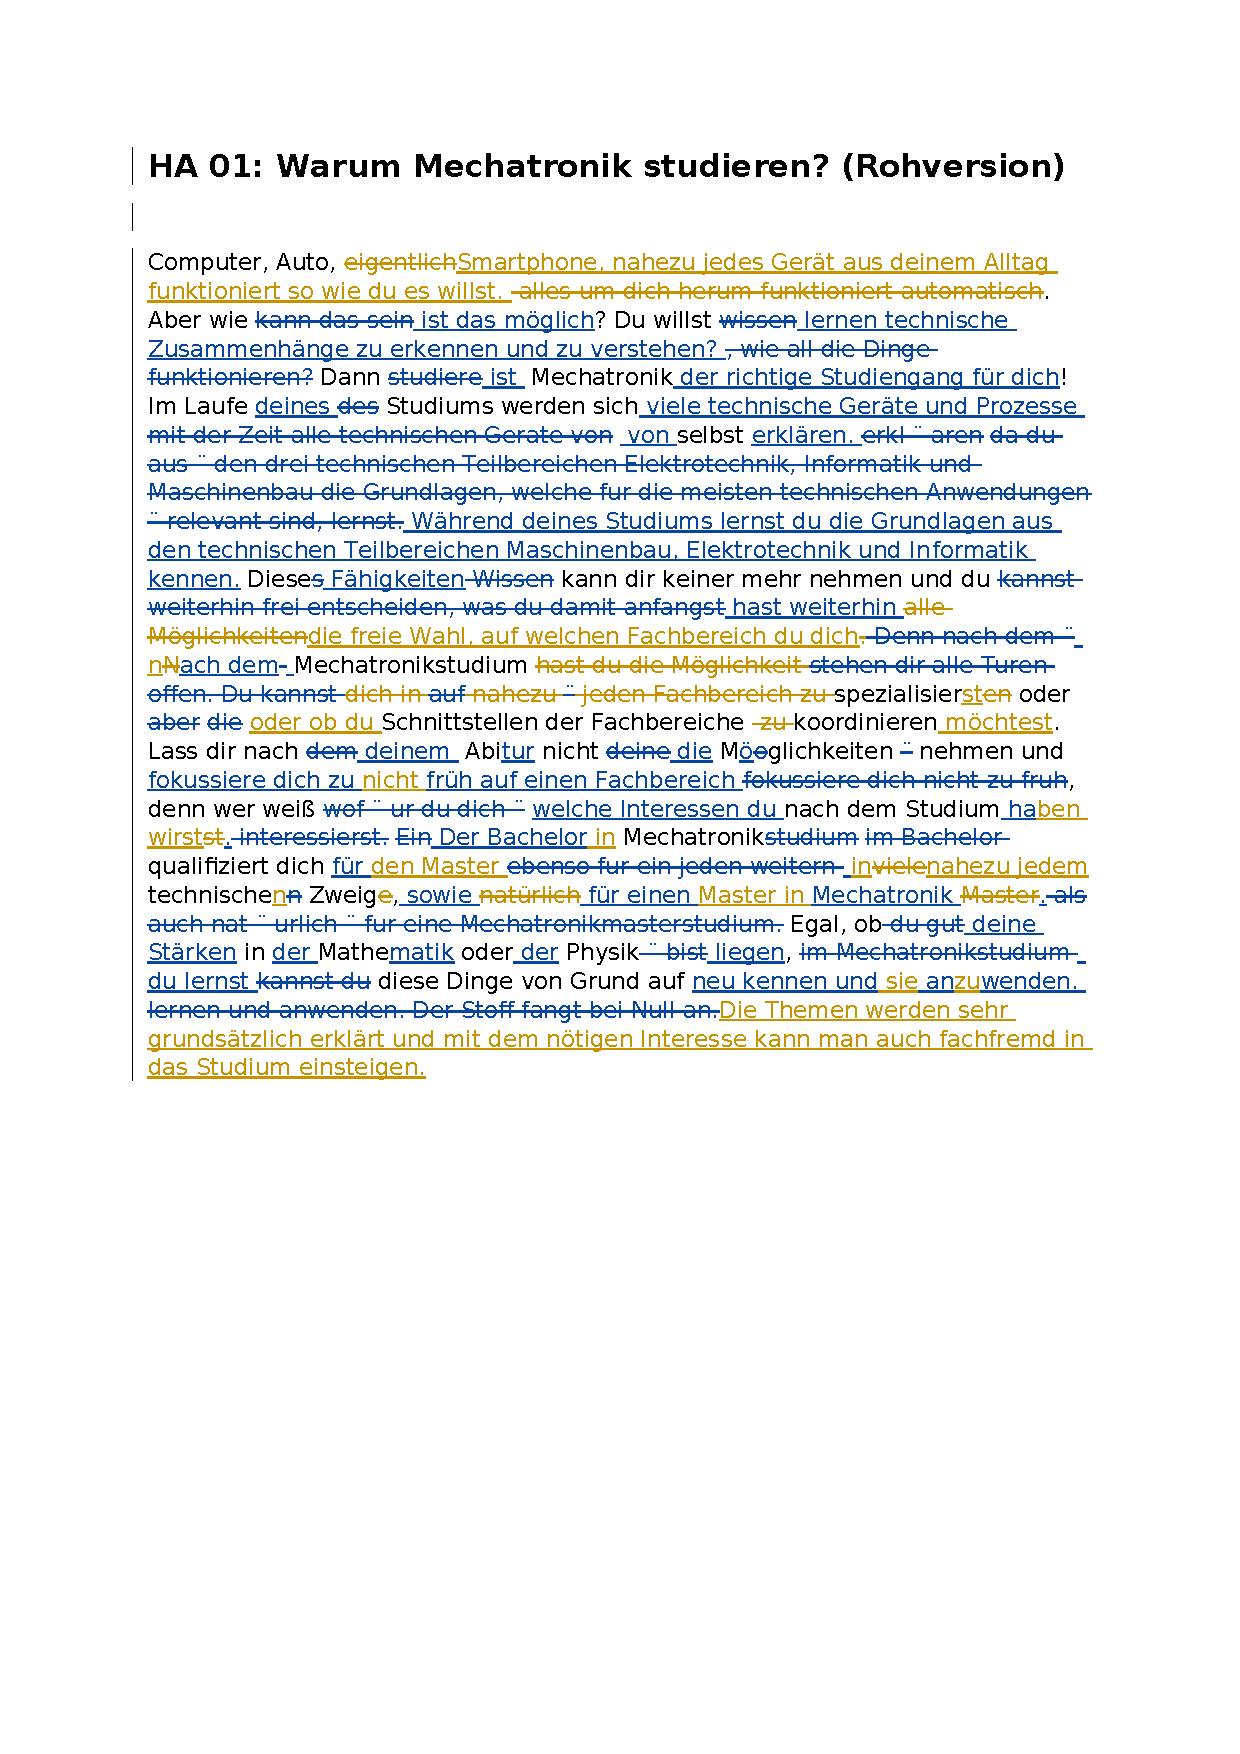
\includepdf[pages=-]{./Hausaufgaben/1_Warum_Mechatronik_studieren/Warum_Mechatronik_Johannes_Rohversion.pdf}
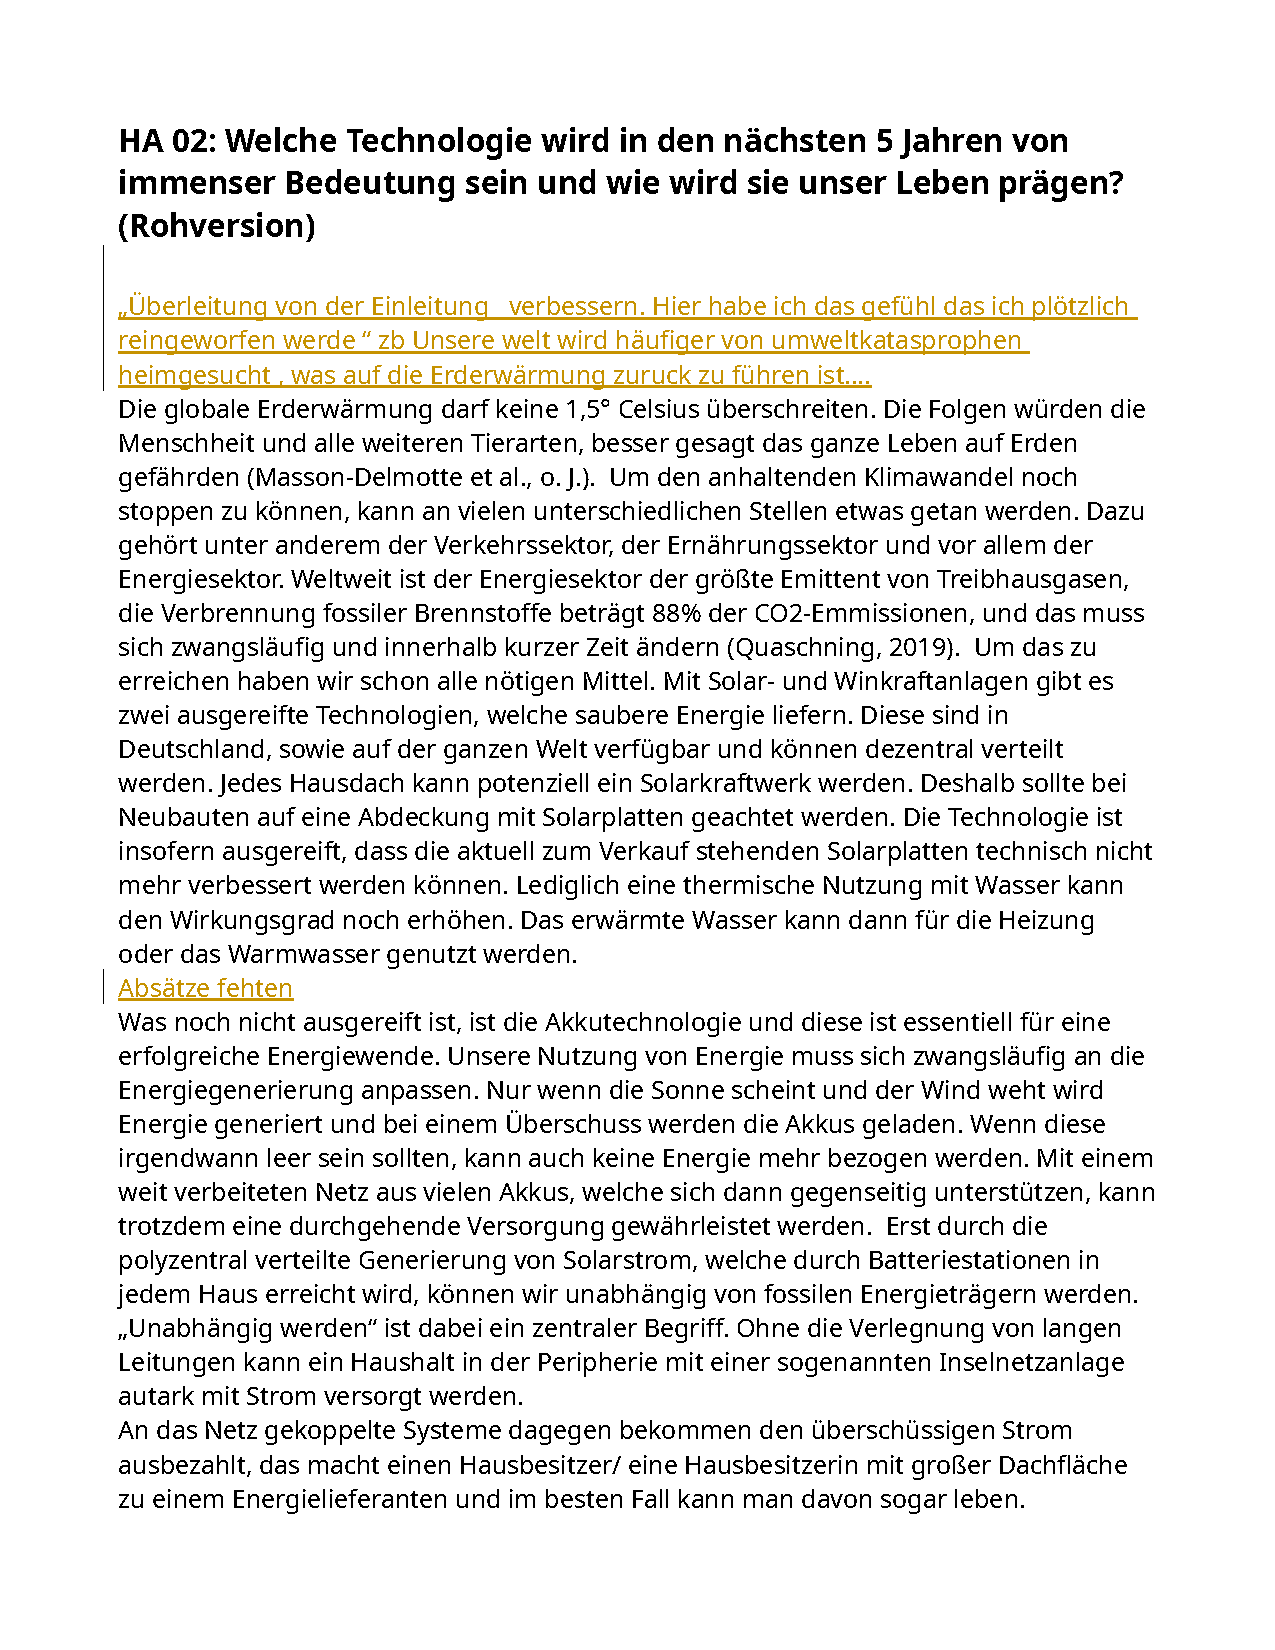
\includepdf[pages=-]{./Hausaufgaben/2_Zukunftstechnologie/Technologie_Johannes_Rohversion.pdf}
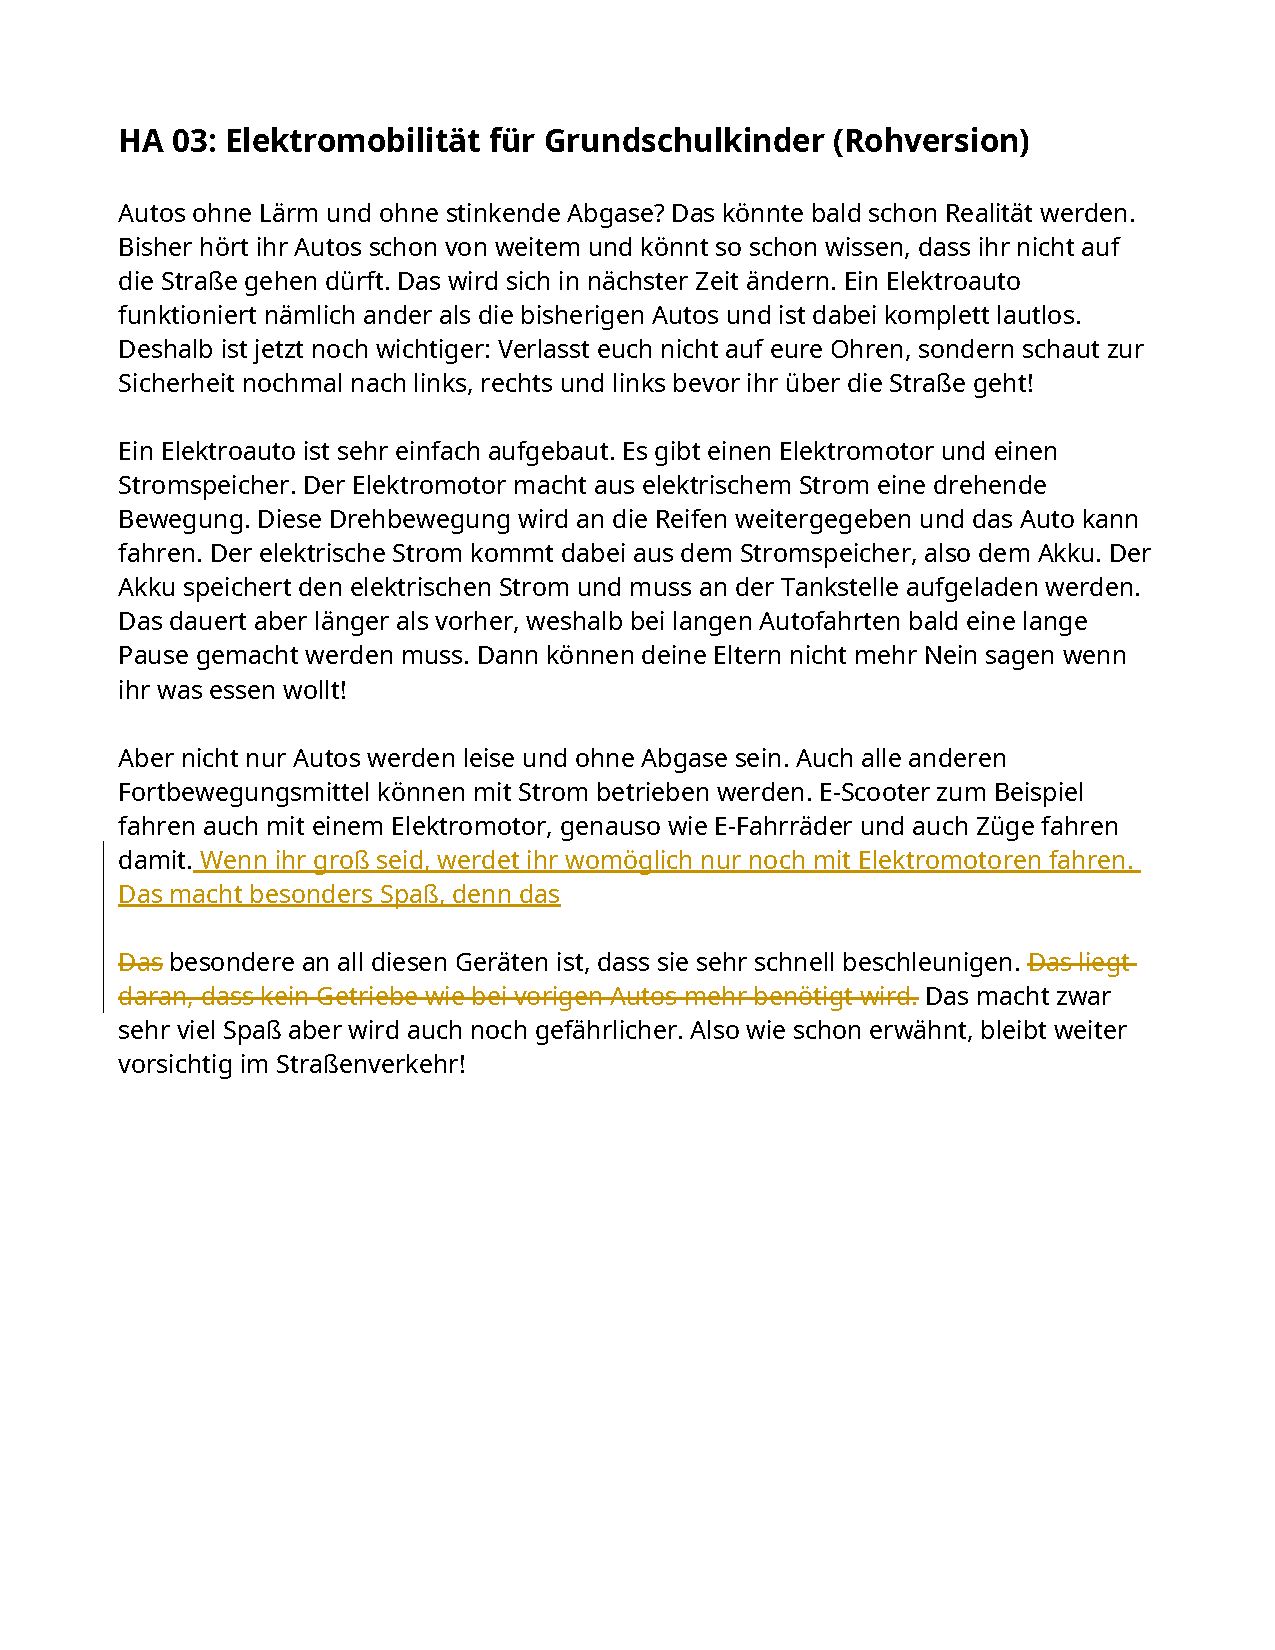
\includepdf[pages=-]{./Hausaufgaben/3_Elektromobilitaet/Elektromobilitaet_Johannes_Rohversion.pdf}
%TODO 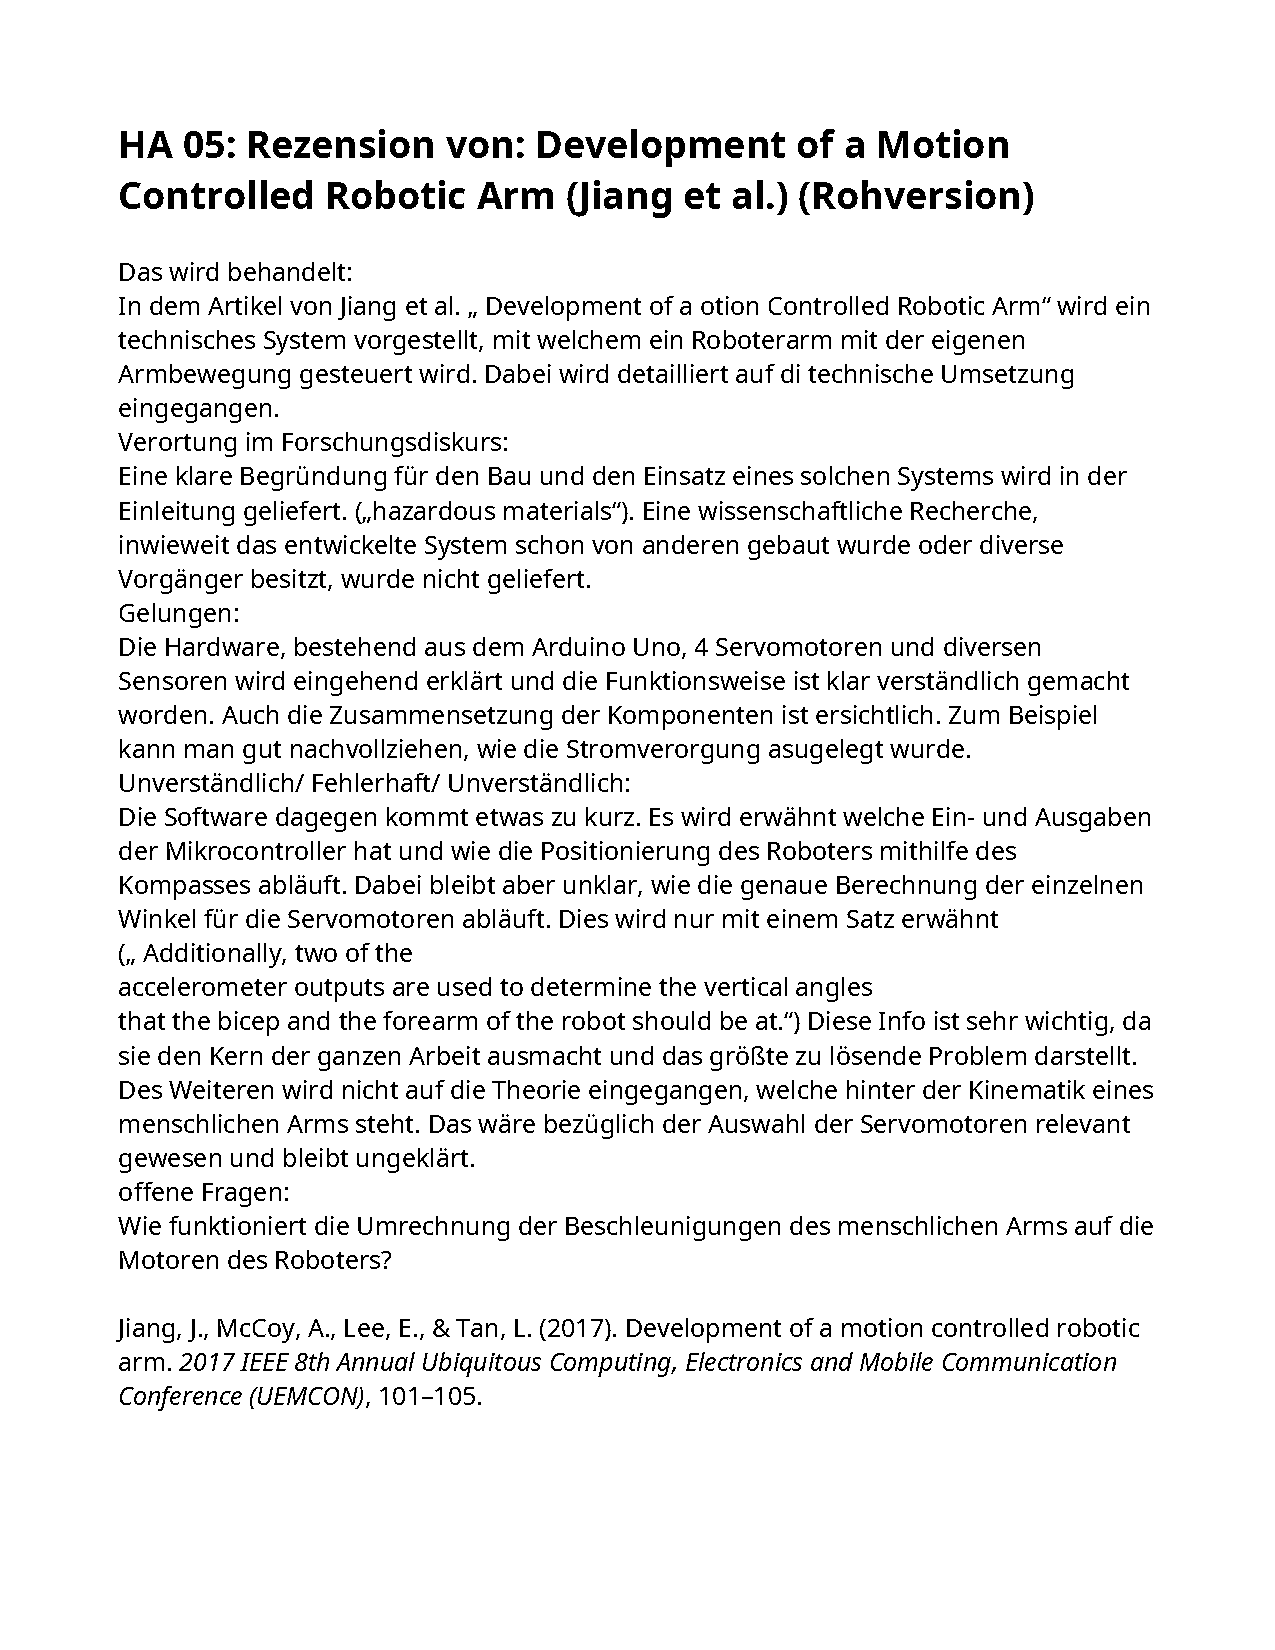
\includepdf[pages=-]{./Hausaufgaben/4_erneuerbare_energien
\includepdf[pages=-]{./Hausaufgaben/5_Artikelrezension/Artikelrezension_Johannes_Rohversion.pdf}
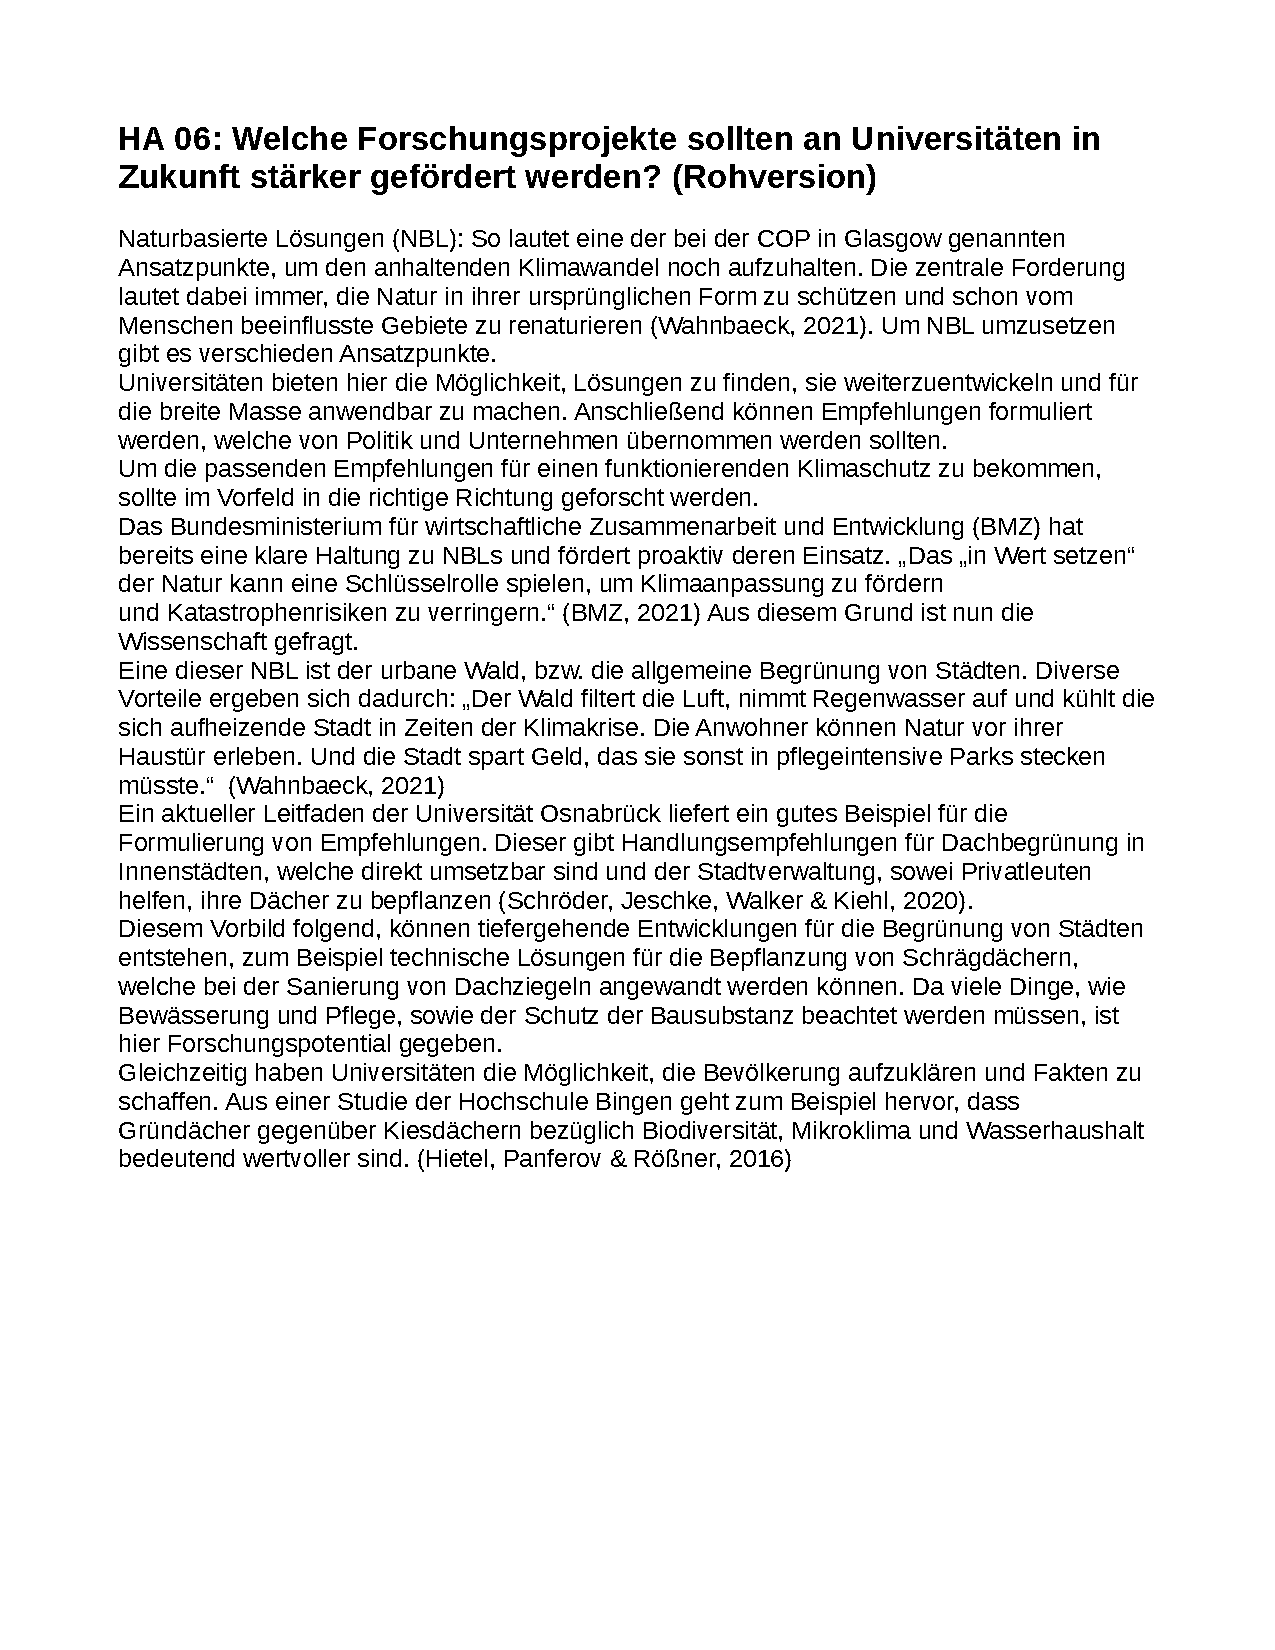
\includepdf[pages=-]{./Hausaufgaben/6_Forschungsprojekte/Forschungsprojekte_Johannes_Rohversion.pdf}
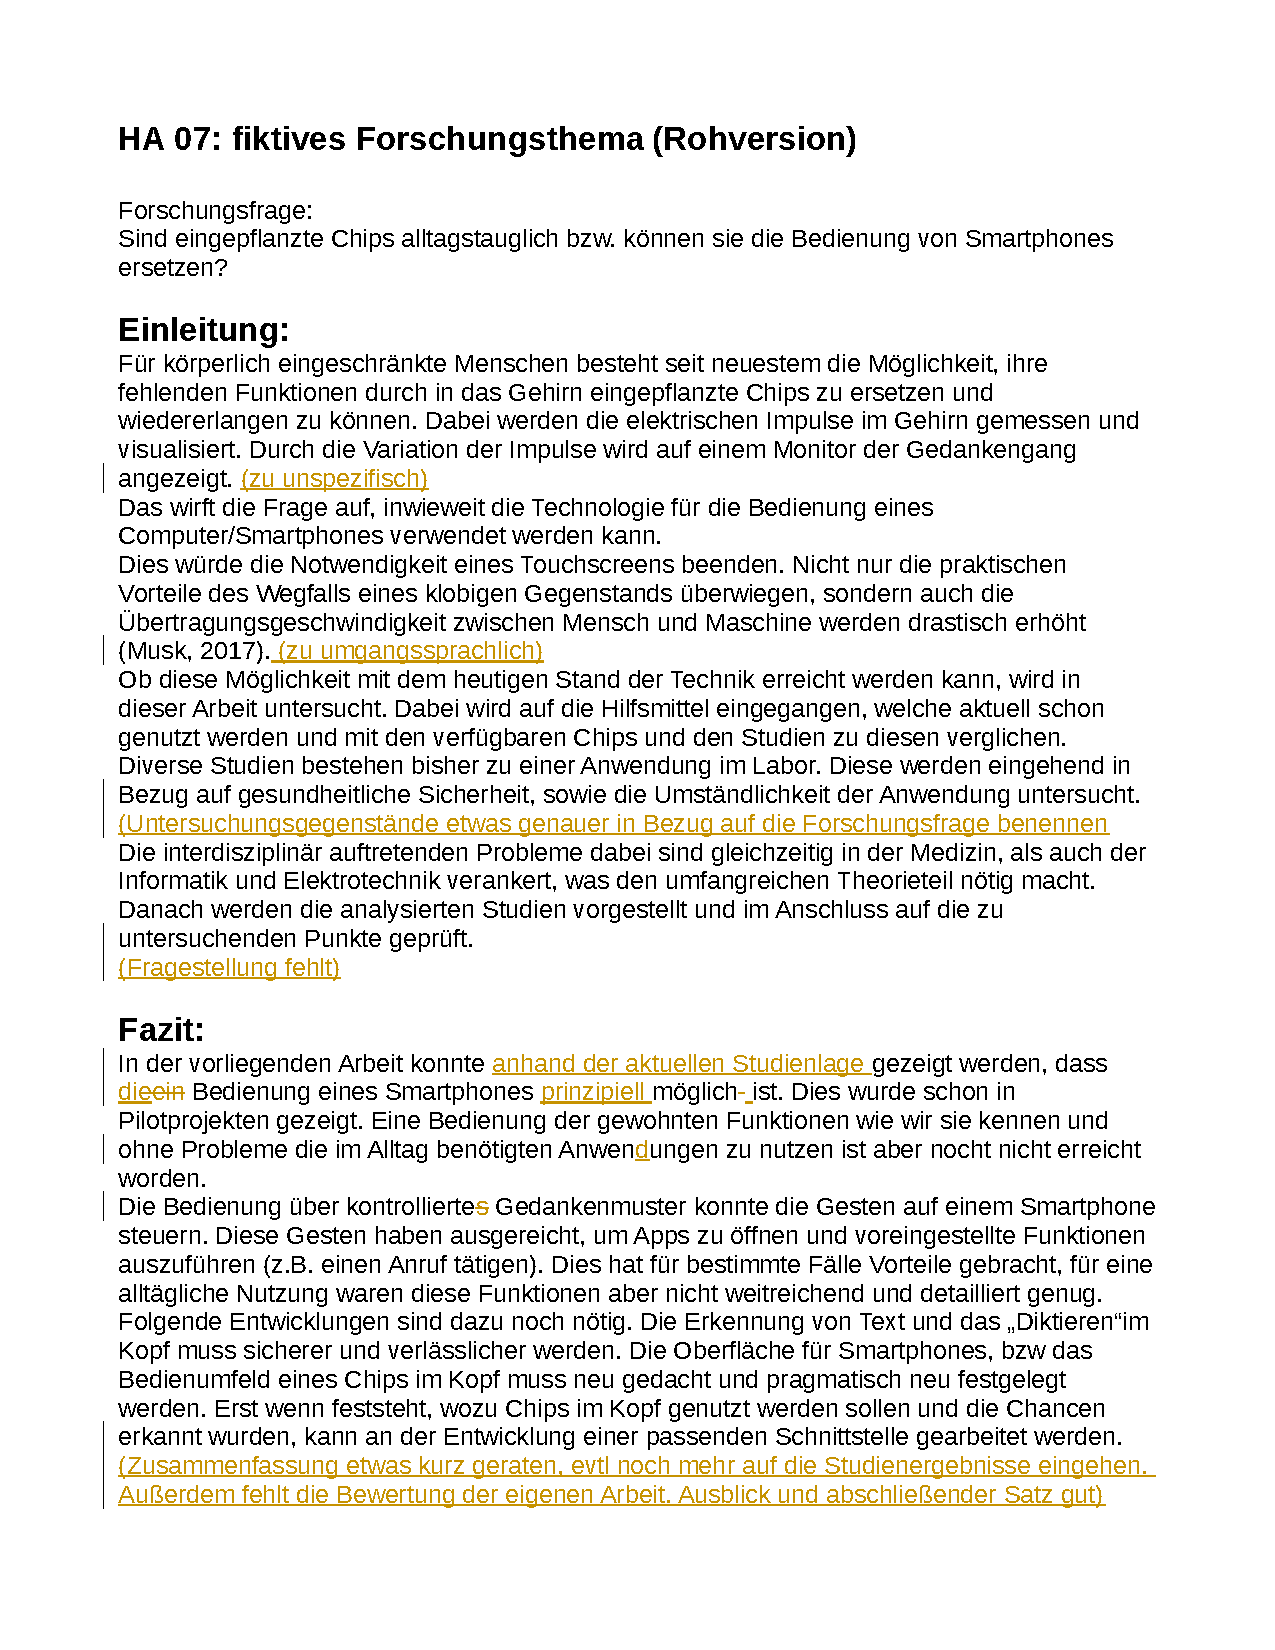
\includepdf[pages=-]{./Hausaufgaben/7_fikt_Forschungsarbeit/Forschungsthema.pdf}
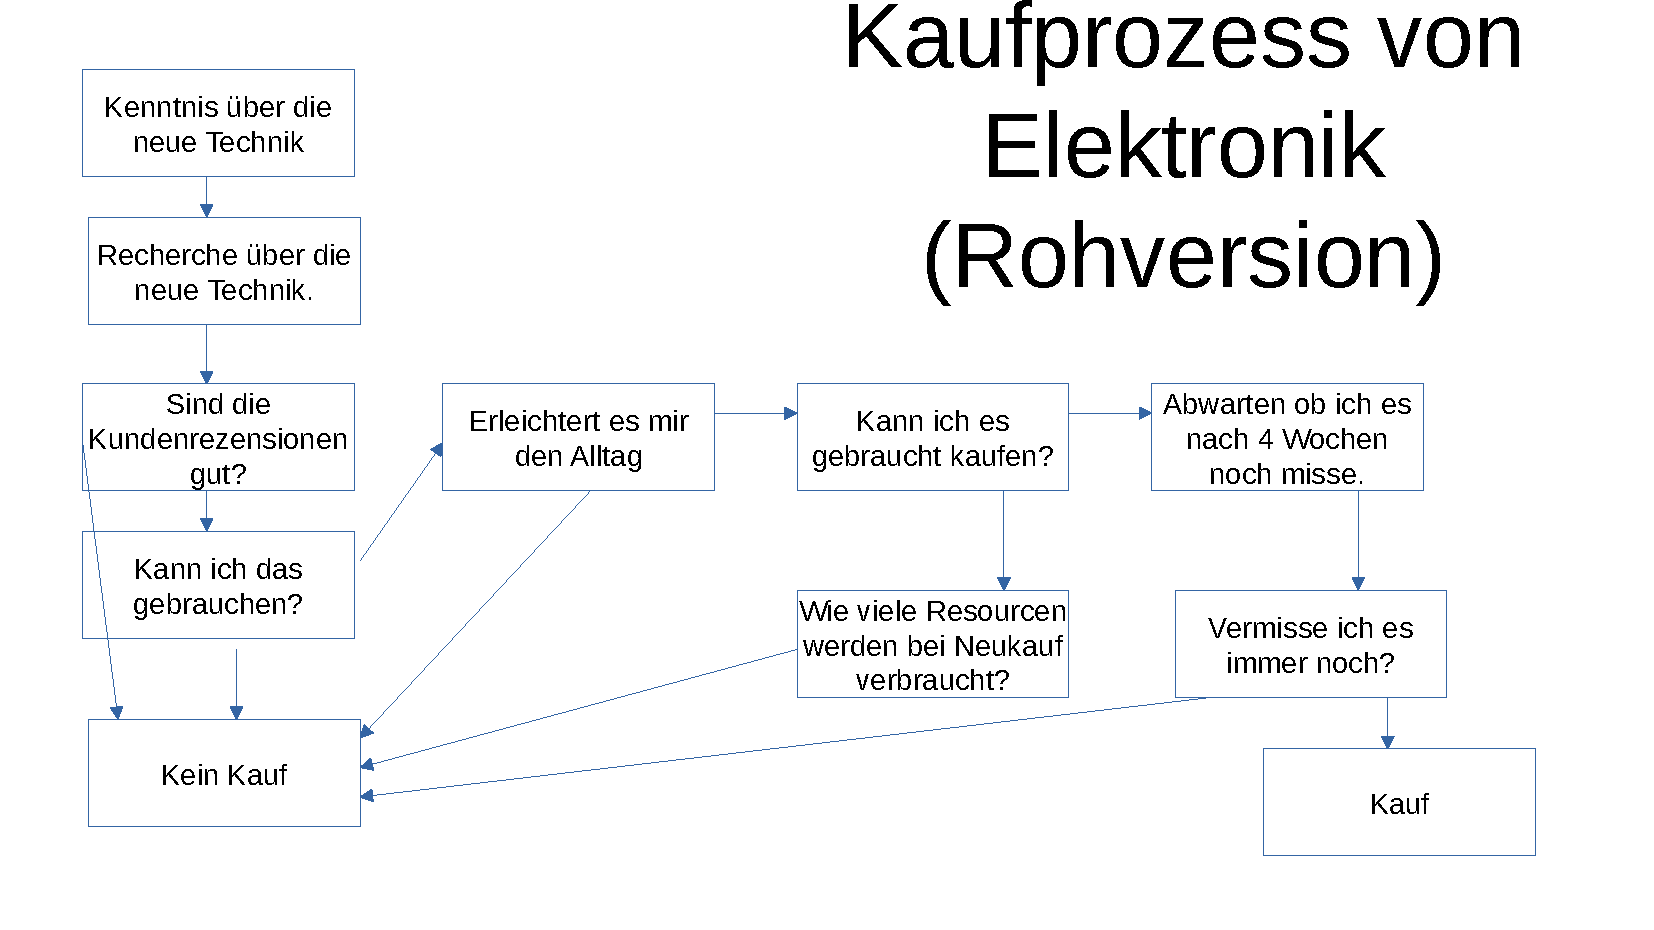
\includepdf[pages=-]{./Hausaufgaben/8_Kaufprozess/Kaufprozess_Grafik_Rohversion.pdf}
\end{document}
